
\documentclass[journal,12pt,twocolumn]{IEEEtran}
\usepackage{setspace}
\usepackage{gensymb}
\singlespacing
\usepackage[cmex10]{amsmath}
\usepackage{amsthm}
\usepackage{mathrsfs}
\usepackage{txfonts}
\usepackage{stfloats}
\usepackage{bm}
\usepackage{cite}
\usepackage{cases}
\usepackage{subfig}
\usepackage{longtable}
\usepackage{multirow}
\usepackage{enumitem}
\usepackage{mathtools}
\usepackage{steinmetz}
\usepackage{tikz}
\usepackage{circuitikz}
\usepackage{verbatim}
\usepackage{tfrupee}
\usepackage[breaklinks=true]{hyperref}
\usepackage{graphicx}
\usepackage{tkz-euclide}
\usetikzlibrary{calc,math}
\usepackage{listings}
    \usepackage{color}                                            %%
    \usepackage{array}                                            %%
    \usepackage{longtable}                                        %%
    \usepackage{calc}                                             %%
    \usepackage{multirow}                                         %%
    \usepackage{hhline}                                           %%
    \usepackage{ifthen}                                           %%
    \usepackage{lscape}     
\usepackage{multicol}
\usepackage{chngcntr}
\DeclareMathOperator*{\Res}{Res}
\newcommand{\myvec}[1]{\ensuremath{\begin{pmatrix}#1\end{pmatrix}}}
\renewcommand\thesection{\arabic{section}}
\renewcommand\thesubsection{\thesection.\arabic{subsection}}
\renewcommand\thesubsubsection{\thesubsection.\arabic{subsubsection}}
\renewcommand\thesectiondis{\arabic{section}}
\renewcommand\thesubsectiondis{\thesectiondis.\arabic{subsection}}
\renewcommand\thesubsubsectiondis{\thesubsectiondis.\arabic{subsubsection}}
\hyphenation{op-tical net-works semi-conduc-tor}
\def\inputGnumericTable{}                                 %%
\lstset{
%language=C,
frame=single, 
breaklines=true,
columns=fullflexible
}
\begin{document}
\newtheorem{theorem}{Theorem}[section]
\newtheorem{problem}{Problem}
\newtheorem{proposition}{Proposition}[section]
\newtheorem{lemma}{Lemma}[section]
\newtheorem{corollary}[theorem]{Corollary}
\newtheorem{example}{Example}[section]
\newtheorem{definition}[problem]{Definition}
\newcommand{\BEQA}{\begin{eqnarray}}
\newcommand{\EEQA}{\end{eqnarray}}
\newcommand{\define}{\stackrel{\triangle}{=}}
\bibliographystyle{IEEEtran}
\providecommand{\mbf}{\mathbf}
\providecommand{\pr}[1]{\ensuremath{\Pr\left(#1\right)}}
\providecommand{\qfunc}[1]{\ensuremath{Q\left(#1\right)}}
\providecommand{\sbrak}[1]{\ensuremath{{}\left[#1\right]}}
\providecommand{\lsbrak}[1]{\ensuremath{{}\left[#1\right.}}
\providecommand{\rsbrak}[1]{\ensuremath{{}\left.#1\right]}}
\providecommand{\brak}[1]{\ensuremath{\left(#1\right)}}
\providecommand{\lbrak}[1]{\ensuremath{\left(#1\right.}}
\providecommand{\rbrak}[1]{\ensuremath{\left.#1\right)}}
\providecommand{\cbrak}[1]{\ensuremath{\left\{#1\right\}}}
\providecommand{\lcbrak}[1]{\ensuremath{\left\{#1\right.}}
\providecommand{\rcbrak}[1]{\ensuremath{\left.#1\right\}}}
\theoremstyle{remark}
\newtheorem{rem}{Remark}
\newcommand{\sgn}{\mathop{\mathrm{sgn}}}
\providecommand{\abs}[1]{\vert#1\vert}
\providecommand{\res}[1]{\Res\displaylimits_{#1}} 
\providecommand{\norm}[1]{\Vert#1\rVert}
%\providecommand{\norm}[1]{\lVert#1\rVert}
\providecommand{\mtx}[1]{\mathbf{#1}}
\providecommand{\mean}[1]{E[ #1 ]}
\providecommand{\fourier}{\overset{\mathcal{F}}{ \rightleftharpoons}}
%\providecommand{\hilbert}{\overset{\mathcal{H}}{ \rightleftharpoons}}
\providecommand{\system}{\overset{\mathcal{H}}{ \longleftrightarrow}}
	%\newcommand{\solution}[2]{\textbf{Solution:}{#1}}
\newcommand{\solution}{\noindent \textbf{Solution: }}
\newcommand{\cosec}{\,\text{cosec}\,}
\providecommand{\dec}[2]{\ensuremath{\overset{#1}{\underset{#2}{\gtrless}}}}
\newcommand{\myvec}[1]{\ensuremath{\begin{pmatrix}#1\end{pmatrix}}}
\newcommand{\mydet}[1]{\ensuremath{\begin{vmatrix}#1\end{vmatrix}}}
\numberwithin{equation}{subsection}
\makeatletter
\@addtoreset{figure}{problem}
\makeatother
\let\StandardTheFigure\thefigure
\let\vec\mathbf
\renewcommand{\thefigure}{\theproblem}
\def\putbox#1#2#3{\makebox[0in][l]{\makebox[#1][l]{}\raisebox{\baselineskip}[0in][0in]{\raisebox{#2}[0in][0in]{#3}}}}
     \def\rightbox#1{\makebox[0in][r]{#1}}
     \def\centbox#1{\makebox[0in]{#1}}
     \def\topbox#1{\raisebox{-\baselineskip}[0in][0in]{#1}}
     \def\midbox#1{\raisebox{-0.5\baselineskip}[0in][0in]{#1}}
\vspace{3cm}
\title{ASSIGNMENT-5}
\author{G.Soujanya}
\maketitle
\newpage
\bigskip
\renewcommand{\thefigure}{\theenumi}
\renewcommand{\thetable}{\theenumi}
Download all python codes from 
\begin{lstlisting}
https://github.com/behappy0604/Summer-Internship-IITH/tree/main/Assignment-5
\end{lstlisting}
%
and latex-tikz codes from 
%
\begin{lstlisting}
https://github.com/behappy0604/Summer-Internship-IITH/tree/main/Assignment-5
\end{lstlisting}
%
\section{Question No. 2.70 (b)} 
Find the equation of the Parabola that satisfy the following condition:
Focus $\myvec{0\\-3}$, Directrix $\myvec{0 & 1}$= 3
\section{Solution}
\begin{enumerate}
\begin{lemma}
\label{lemma}
Parabola is a conic whose eccentricity, e=1
\end{lemma}
\begin{lemma}
\label{lemma}
The distance of a point $\vec{P}$ from a line $\vec{n}^T\vec{x}=c$ is given by:
\begin{align}
\frac{\abs{c-\vec{P}^T\vec{n}}}{\norm{\vec{n}}}   
\end{align}
\end{lemma}
\begin{lemma}
The equation for parabola assuming $\lambda=\norm{\vec{n}}^2$ will be: 
\begin{align}
\vec{x}^T(\lambda\vec{I}-\vec{n}\vec{n}^T)\vec{x}+2(c\vec{n}-\lambda\vec{F})^T\vec{x}+\lambda\norm{\vec{F}}^2-c^2&=0\label{eq:2}
\end{align}
\end{lemma}
Given information:
\begin{align}
\vec{F}=\myvec{0\\-3},
\vec{n}=\myvec{0\\1},
c=3,
\lambda=1\label{eq:3}
\end{align}
Substituting values of $\vec{F},\vec{n}$,c,$\lambda$ from\eqref{eq:3}:
\begin{align}
\vec{x}^T\myvec{1&-1\\0&0}\vec{x}+2\myvec{6&0}\vec{x}+0&=0\label{eq:4}
\end{align}
Replacing $\vec{x}$ by $\myvec{x\\y}$ in \eqref{eq:4} gives:
\begin{align}
y^2=-12x
\end{align}
The general equation of parabola we got in \eqref{eq:2} is of form:
\begin{align}
\vec{x}^T\vec{V}\vec{x}+2\vec{u}^T\vec{x}+f=0
\end{align}
\begin{align}
\vec{V}=\lambda\vec{I}-\vec{n}\vec{n}^T\\
\vec{u}=c\vec{n}-\lambda\vec{F}\\
f=\lambda\norm{\vec{F}}^2-c^2
\end{align}
$\vec{n}=\myvec{x\\y}$,$\lambda=\norm{\vec{n}}^2=x^2+y^2$; $\vec{I}=\myvec{1&0\\0&1}$.Now,
\begin{align}
\mydet{\vec{V}}&=\mydet{\lambda-x^2&-xy\\-xy&\lambda-y^2}\\
&=\mydet{y^2&-xy\\-xy&x^2}\\
&=0\label{eq:12}
\end{align}
Also characteristic equation of $\vec{V}$ is given by:
\begin{align}
\mydet{\alpha\vec{I}-\vec{V}}=0\\
\mydet{\alpha-\ambda+x^2&xy\\xy&\alpha-\lambda+y^2}=0\\
\mydet{\alpha-y^2&xy\\xy&\alpha-x^2}=0\\
\alpha^2-\alpha(x^2+y^2)=0\\
\alpha(\alpha-\lambda)=0\\
\alpha_{1}=0\label{eq:18}\\
\alpha_{2}=\lambda=x^2+y^2=\norm{\vec{n}}^2
\end{align}
So, \eqref{eq:12} and \eqref{eq:18} shows that \eqref{eq:2} is an equation of parabola.
\end{enumerate}
\numberwithin{figure}{section}
\begin{figure}[!ht]
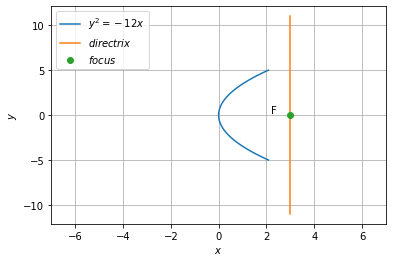
\includegraphics[ width=\columnwidth]{download (3).png}
\caption{Parabola}
\label{fig:Parabola}	
\end{figure}
\end{document}
© 2021 GitHub, Inc.